%% Generated from results/shortlist.csv. Do not edit by hand.
\begin{figure}[t]
\centering
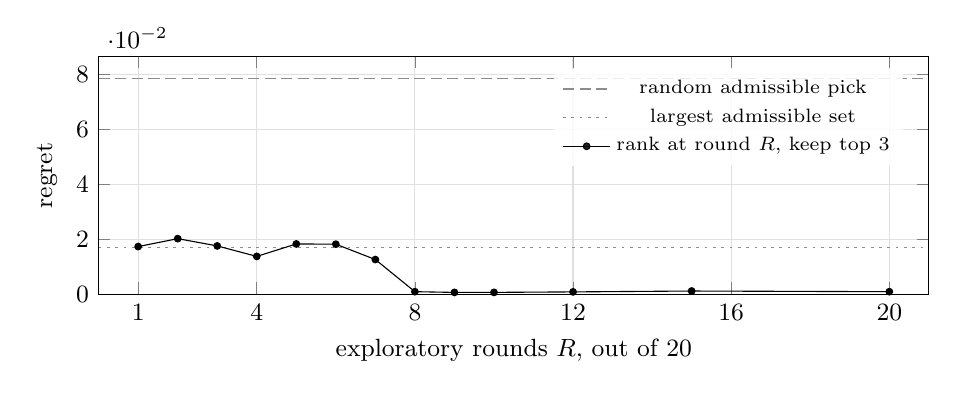
\begin{tikzpicture}
\begin{axis}[
  width=\columnwidth, height=46mm,
  xlabel={exploratory rounds $R$, out of 20},
  ylabel={regret}, ylabel near ticks,
  xmin=0, xmax=21, ymin=0,
  xtick={1,4,8,12,16,20},
  label style={font=\small}, tick label style={font=\small},
  legend style={font=\scriptsize, at={(0.97,0.95)},
    anchor=north east, draw=none, fill=white,
    fill opacity=0.85, text opacity=1},
  grid=major, grid style={black!12},
]
\addplot[black!45, dash pattern=on 4pt off 2pt, no markers] coordinates {(0,0.078668) (21,0.078668)};
\addlegendentry{random admissible pick}
\addplot[black!45, dash pattern=on 1pt off 2pt, no markers] coordinates {(0,0.017162) (21,0.017162)};
\addlegendentry{largest admissible set}
\addplot[black, mark=*, mark size=1.2pt] coordinates {(1,0.017381) (2,0.020263) (3,0.017619) (4,0.013800) (5,0.018337) (6,0.018244) (7,0.012656) (8,0.000956) (9,0.000687) (10,0.000700) (12,0.000875) (15,0.001194) (20,0.000950)};
\addlegendentry{rank at round $R$, keep top 3}
\end{axis}
\end{tikzpicture}
\caption{Regret falls to the full budget's level by round eight.}
\label{fig:costfidelity}
\end{figure}
